\section{Tutorial \textit{Forking}}
    Esta seção mostra os procedimentos realizados durante a leitura do tutorial \href{https://guides.github.com/activities/forking/}{\textit{"Forking projects"}}.
    
    \subsection{Realizando \textit{fork}}
    Para realizar o tutorial, foi necessário utilizar minha conta no Github e dar \textit{fork} no repositório \textit{Spoon-Knife} armazenado em https://github.com/octocat/Spoon-Knife.
    
    \begin{figure}[H]
        \caption{\textit{Fork} no repositório \textit{Spoon-knife}}
        \vspace{0.5cm}
        \centering
        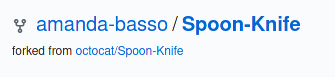
\includegraphics[width=5cm]{imagens/fork.png}
        \label{figura:fork}
    \end{figure}

    \subsection{Realizando modificações, \textit{push} e abrindo \textit{pull request}}
    Modifiquei parte do texto do arquivo \textit{index.html} apenas para efeitos de prática do tutorial. Em seguida, dei \textit{push} para o repositório \textit{forked} - aquele que fica armazenado na minha conta \textit{Github}. Por último, abri um \textit{pull request} para o \textit{branch master} do repositório original.
    \begin{figure}[H]
        \caption{\textit{Pull request} para o repositório base}
        \vspace{0.5cm}
        \centering
        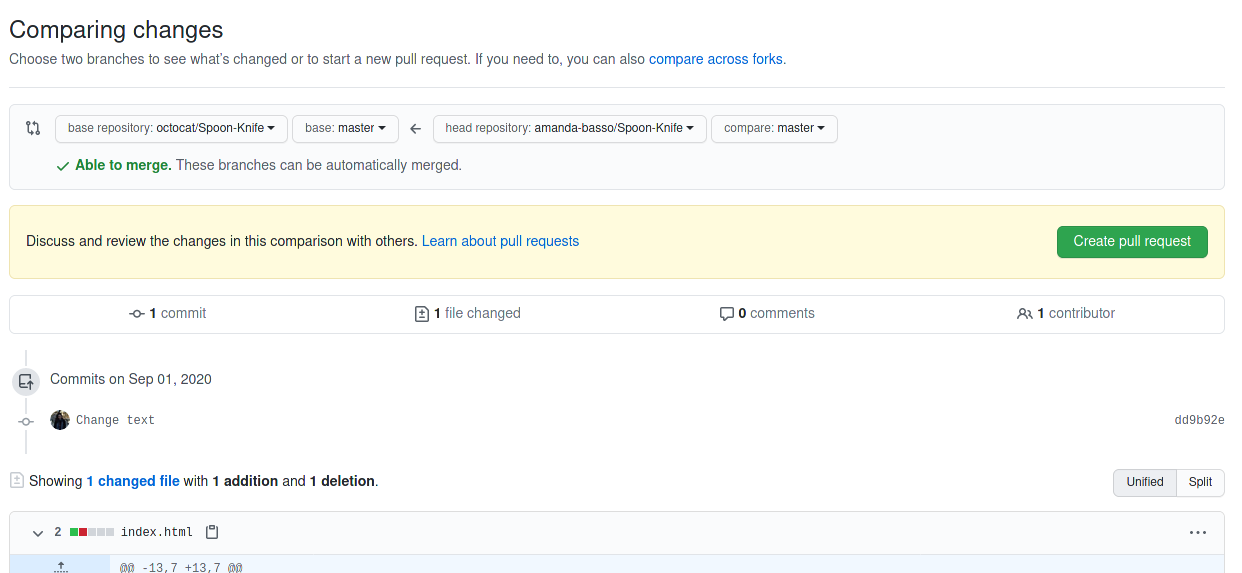
\includegraphics[width=15cm]{imagens/pull_request_fork.png}
        \label{figura:pull_request_fork}
    \end{figure}

    A imagem\ref{figura:result_fork} mostra o \textit{pull request}.
    
    \begin{figure}[H]
        \caption{\textit{Pull request}}
        \vspace{0.5cm}
        \centering
        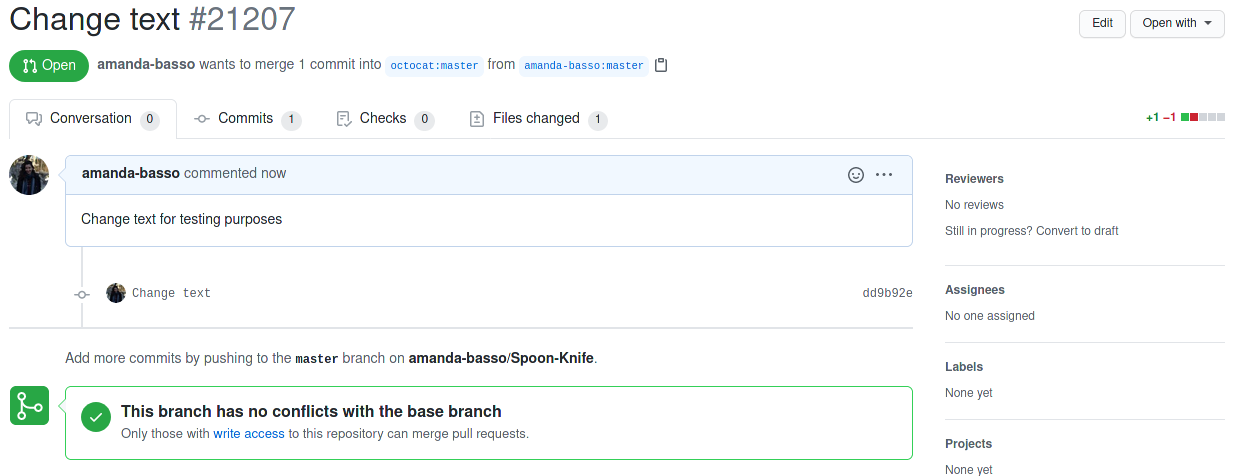
\includegraphics[width=15cm]{imagens/result_fork.png}
        \label{figura:result_fork}
    \end{figure}
